
%%% Local Variables:
%%% mode: latex
%%% TeX-master: "../../doktorarbeit"
%%% End:
\chapter{The effects of rotation}
In this chapter we study the effects rotation have on the GW signal. 
We present three models based on the same progenitor, two rotating models and one non-rotating.
This allows us to study how the signal GW is effected by rotation. 


\section{Supernova Models}
We present the GW signal from three models based on the progenitor of
\cite{heger_05}, which is a solar-metallicity star with a ZAMS mass of $15 \msun$.
The progenitor was developed, taking into account the effects of magnetic fields and rotation,
from ZAMS to the onset of iron-core collapse. The inclusion of magnetic fields lead to an overall
reduction of the final rotation rate of the iron core, compared to a star evolved without magnetic
fields. The main difference between the three models is their rotation profiles. One of the models
uses the profile of the progenitor (m15r), an other has a enhanced rotation profile (m15fr),
in the last model the rotation rate has been set to zero throughout the star (m15nr)
In \fig{figp2:rot} we show the rotation profiles of m15fr and m15fr.
\begin{figure}           
\centering                            
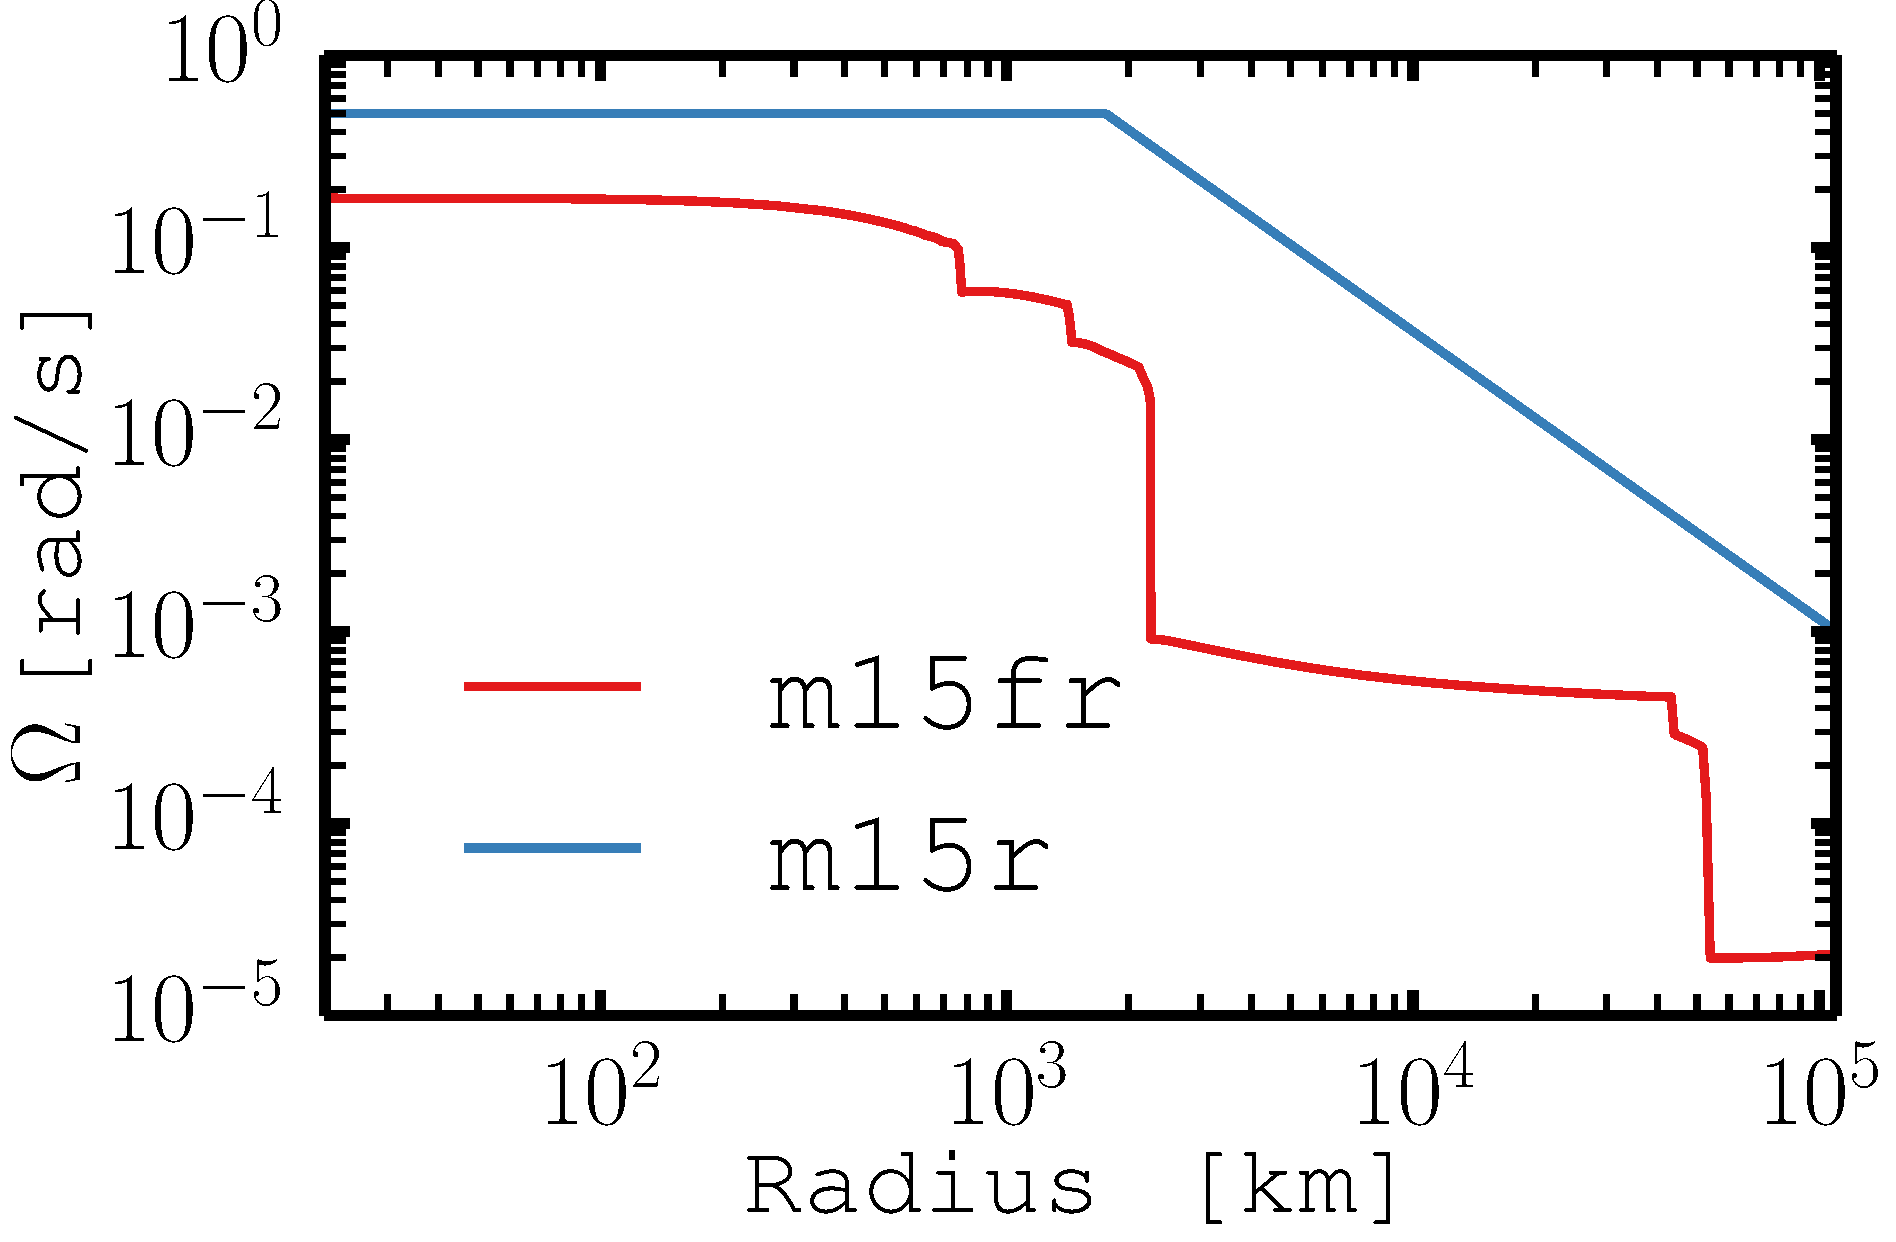
\includegraphics[width=0.9\textwidth]{./images/paper2/rot.pdf}
\caption{The radial rotation profiles for the two rotating models. The red represents model 
m15fr and the blue line represents m15r. \label{figp2:rot}}
\end{figure}
\begin{itemize}
\item \textbf{m15r:} 
\item \textbf{s20:}
\item \textbf{s20s:} 
\end{itemize}
